\documentclass{article}
\usepackage{graphicx}
\usepackage{float}

\begin{document}

If you are lost, you can look at this helpful map (figure \ref{fig:theuniverse}) to find where you are!

\begin{figure}[H] % The [H] provides exact positioning.
    \centering
    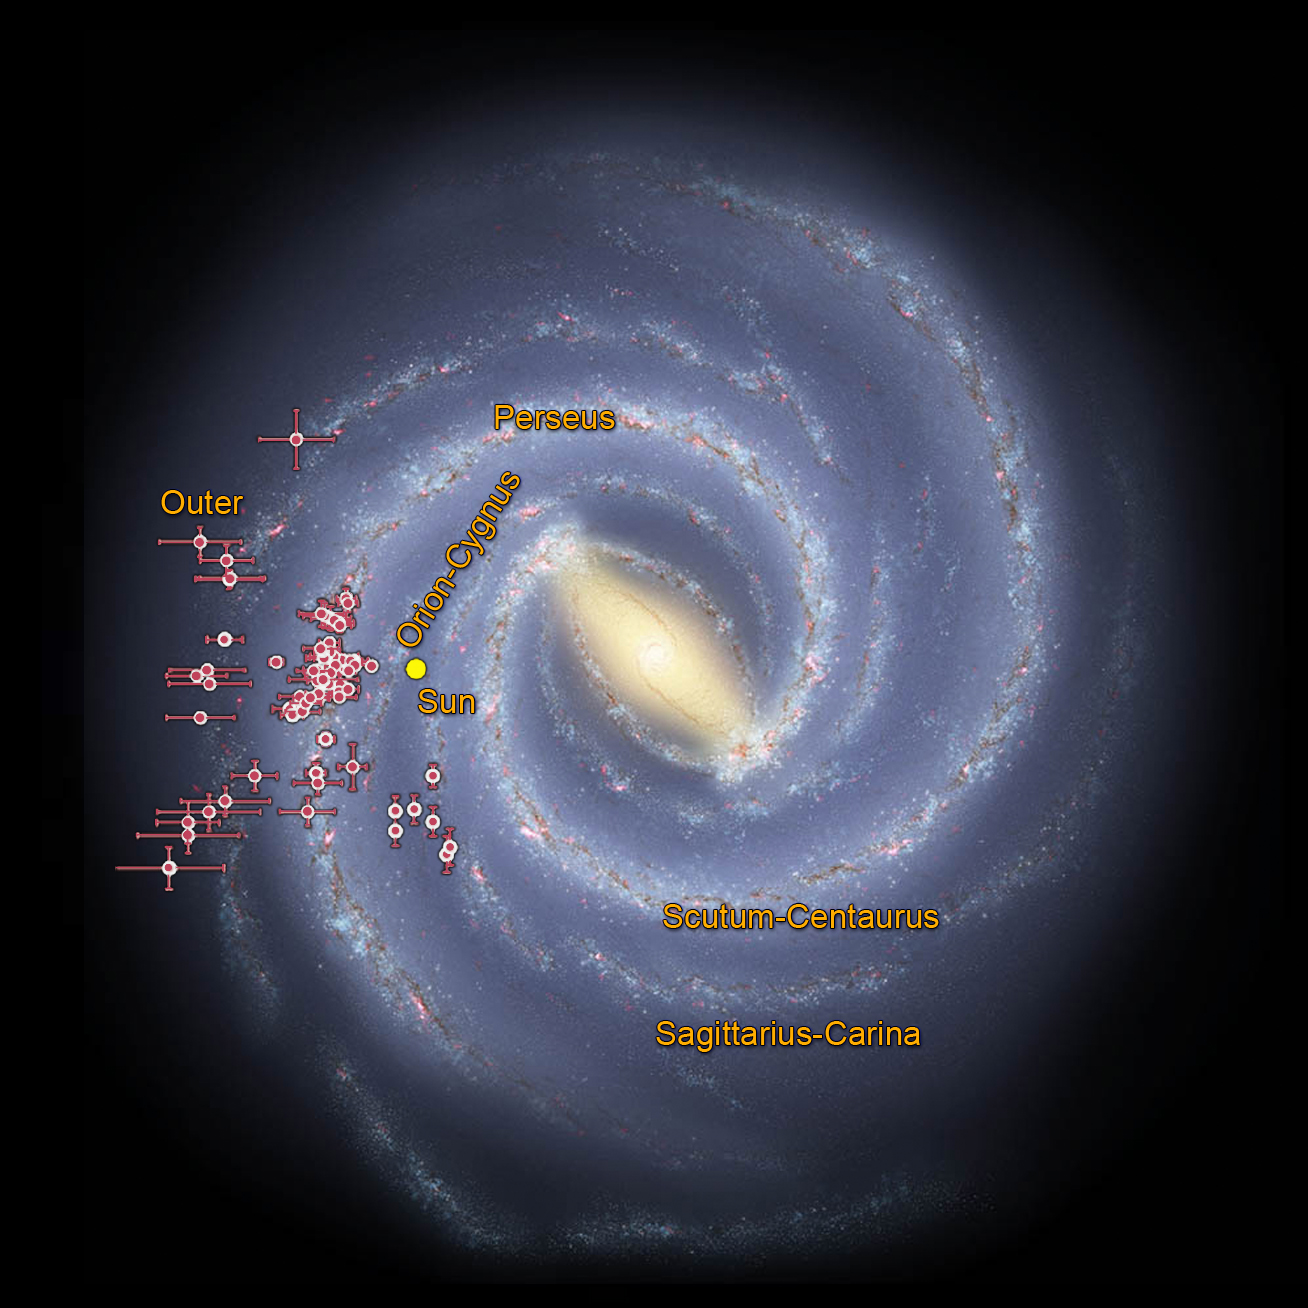
\includegraphics[width=\linewidth]{theuniverse.jpg}
    \caption{The Universe}
    \label{fig:theuniverse}
\end{figure}

If you remove the \verb|[H]|, then \LaTeX{} will probably move the figure to not be in the middle of this text! Also, check out table \ref{tab:mytable}!

\begin{table}[H]
    \centering
    \begin{tabular}{r|ccll}
        Foo & bar & bat & baz & fizz \\\hline
        buzz & fizzbuzz & & one & two \\
        three & four & five & six & seven \\
    \end{tabular}
    \caption{The Best Table Ever Made!}
    \label{tab:mytable}
\end{table}


\end{document}